\documentclass[9pt, mathserif]{beamer}
\usefonttheme{serif}
\usetheme{Berlin}
\usecolortheme{seagull}
\usepackage[utf8]{inputenc}
\usepackage{amsfonts}
\usepackage{lmodern}
\usepackage{amsmath}
\usepackage{geometry}
\usepackage{graphicx}
\usepackage{tikz}
\usepackage{url}
\usepackage{geometry}
\usepackage{bm}
\usepackage{physics}
\usepackage{float}
\usepackage{subfigure}
\usepackage{wrapfig}
\usepackage{multirow}
\usepackage{xcolor}
\usepackage{indentfirst}
\usepackage{ragged2e}
\justifying\let\raggedright\justifying
\setlength{\parindent}{2em}


\title{\textbf{\textbf{}}}
\author{\textbf{Xianglong Song}}
\institute{Boling Class of Physics, School of Physics, Nankai University, Tianjin 300071, China}
\date{Jan 25, 2024}

\begin{document}
    \begin{frame}
        \titlepage
        Crab
        naima
        results
        we can save time using SSC in SED
        crab is different because we need SSC
    \end{frame}
    \begin{frame}
		\frametitle{Contents} 
		\tableofcontents
	\end{frame}
    \section{Crab Nebula}
        \begin{frame}
            \frametitle{Introduction}
            \begin{wrapfigure}{r}{0.4\textwidth}
                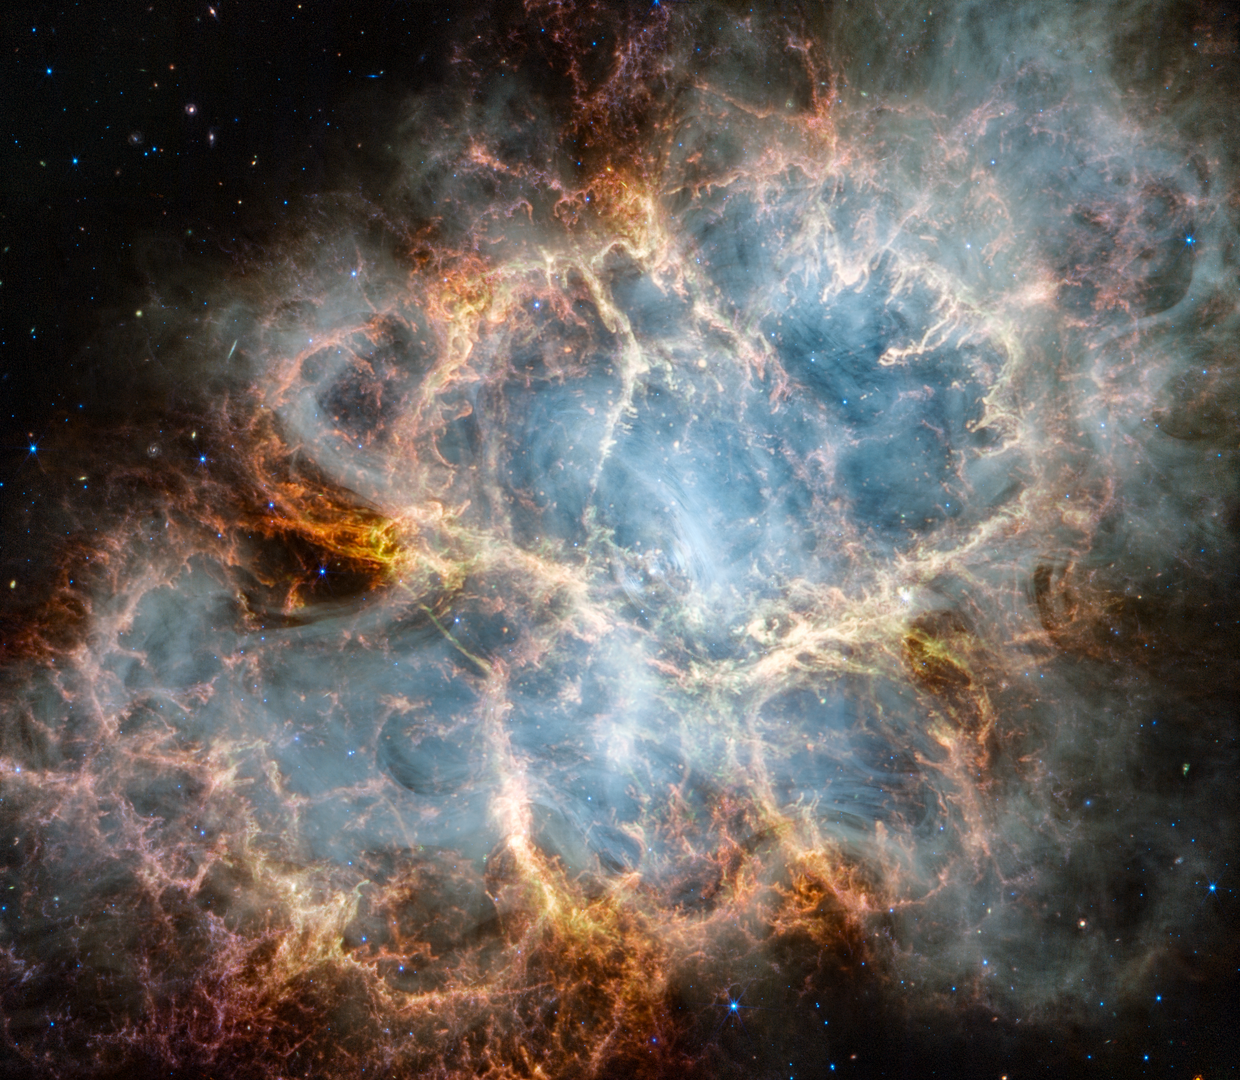
\includegraphics[width=0.4\textwidth]{1240px-Crab_Nebula_imaged_using_James_Webb_Space_Telescope.png}
                \caption{Crab Nebula imaged using James Webb Space Telescope in infrared via its NIRCam (Near-Infrared Camera) and MIRI (Mid-Infrared Instrument).}
            \end{wrapfigure}

            The Crab Nebula (catalogue designations M1, NGC 1952, Taurus A) is a supernova remnant and pulsar wind nebula in the constellation of Taurus.

            In 2019 the Crab Nebula was observed to emit gamma rays in excess of 100 TeV, making it the first identified source beyond 100 TeV.

            \phantom{0}\\
            \phantom{0}\\
            \phantom{0}\\
            \phantom{0}\\
            \phantom{0}\\
            \phantom{0}\\
            \phantom{0}\\
            \phantom{0}\\
            \phantom{0}\\
        \end{frame}

    \section{References}
        \begin{frame}
            \begin{thebibliography}{1}
                \bibitem{bib1}
                1
            \end{thebibliography}
        \end{frame}
\end{document}


